%version of 05-01-20

\chapter{Finding Beauty in Numerical Relationships}
\label{Appendix:Tetra}

In the course of introducing the many mathematical topics that have occupied us throughout the core of our text, we have encountered many instances of ``order" in the world, which some might call ``beauty".  This chapter builds upon instances of beauty that we have uncovered in studying relationships among classes of numbers.

\medskip

In Chapter~\ref{ch:doingmath}, we observed that there is a very compact formula for the sum of the first $n$ positive integers, in the form of a degree-$2$ polynomial which we named $\Delta_n$.  In Chapter~\ref{ch:Summation}, we discovered that the elegance of the expression for $\Delta_n$ extends to the problem of summing the first $n$ perfect squares, and the first $n$ perfect cubes, and so on to higher powers:  For each fixed power $d$, the sum of the first $n$ perfect $d$th powers of positive integers is a polynomial of degree $d+1$.  So, our first search for beauty in numbers uncovered an extension that is based on the degrees of simple polynomials.

\smallskip

We now focus on summing the first $n$ numbers $\Delta_i$ and looking at the sums of those sums---another way to extend beyond the sum of the first $n$ integers.  And we find yet more order and beauty!

\medskip

The reader has probably guessed by this time that our quest for order and beauty is just the ``spoonful of sugar" which accompanies our primary goal---to develop the methodology which enables our quest.  You have surely noted by this point in our joint journey that the activity of solving mathematical problems encompasses several sub-activities which are challenging in their own rights.  One must develop the insights that help one settle on an {\em approach} to the problem---should one strive to represent the problem textually or pictorially \ldots?  And, once having chosen an approach, one must select appropriate {\em tools}---should one seek to argue from small instances to larger ones (induction), should one strive to derive a contradiction based on assuming the negation of one's targeted assertion, and so on?

\smallskip

We hope that our focus in this section on highly structured problems will help the reader gain valuable experience in proceeding through the entire spectrum of activities needed to tackle sophisticated mathematical problems.


%%%%%%%%%%%%%%%%%%%
\section{Revisiting the Triangular Numbers $\Delta_n$}

\index{order-$n$ triangular number} \index{triangular number}

Recall that for each positive integer $n$, the {\it order-$n$ triangular number} is the sum of the  first positive integers: $\Delta_n \ = \ 1 \ + \ 2 \ + \cdots + \ n$.  In Chapter~\ref{ch:Summation}, we derived the value $\Delta_n$, namely ${1 \over 2}n(n+1)$, in several ways, including, notably,
\begin{itemize}
\item
Gauss's ``trick" that builds upon the following invariant: 

For all $k$, the $k$th and $n-k+1$th terms of $\Delta_n$'s defining summation sum to $n+1$ 
\item 
Fubini's double-counting principle, which represents the $k$th integer by $k$ tokens:

Merging two triangle-shaped collections of tokens yields a rectangle of area $n(n+1)$.  Indeed, the representation of $\Delta_n$ by a triangle of tokens is the origin of its ``triangular" name.
\end{itemize}
Fig.~\ref{fig:Tetrahedral2} depicts a stratagem that melds Gauss's and Fubini's.
\begin{figure}[h]
\begin{center}
        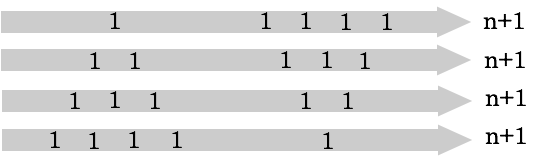
\includegraphics[scale=0.4]{FiguresArithmetic/appTetrahedral2}
        \caption{Computing $\Delta_n$ for $n=4$: Two copies of a triangle are arranged so that all rows have the same sum; i.e., the row-sum is an {\em invariant}.}
        \label{fig:Tetrahedral2}
\end{center}
\end{figure}
The figure's use of invariants will serve as the basic reasoning principle in our expedition beyond $\Delta_n$.


%%%%%%%%%%%%%%%
\section{Tetrahedral Numbers}
\label{sec:tetraedralNumbers}

\index{tetrahedral number} \index{$\widehat{\Theta}_n$: the $n$th tetrahedral number}

This section extends our work on $\Delta_n$.  The extension emerges from the problem of summing the first $n$ triangular numbers, i.e., to evaluate the summation
\[ \widehat{\Theta}_n \ \eqdef \ \Delta_1 \ + \ \Delta_2 \ + \cdots +\ \Delta_n \]
Each such sum is called a {\it tetrahedral number}: the  $n$th sum is denoted $\widehat{\Theta}_n$; see Footnote~\ref{foot:Theta}.  In common with $\Delta_n$'s geometric epithet, ``triangular", the ``tetrahedral" name of $\widehat{\Theta}_n$ calls to mind the number's 3-dimensional representation as a tetrahedron of tokens. 

\subsection{An Algebraic Evaluation of $\widehat{\Theta}_n$}

The most obvious way to evaluate the summation underlying $\widehat{\Theta}_n$ is to replace each $\Delta_k$ by its value ${1 \over 2}k (k+1)$ and to proceed by algebraic manipulations to evaluate the sum of the $n$ triangular numbers.  We leave it to the reader to follow this strategy and verify that
\begin{eqnarray*}
\widehat{\Theta}_n & = & \sum_{k=1}^{n} \ \Delta_k \\
      & = & \sum_{k=1}^{n} \ \frac{1}{2} (k^2 + k) \\
      & =  & \frac{1}{2} \left( \sum_{k=1}^{n} \ k^2 + \sum_{k=1}^{n}  \ k \right) \\
      & = & {1 \over 6} n (n+1)(n+2)
\end{eqnarray*}
The final value comes from invoking Eq.~(\ref{eq:sum-1-to-nsq}) and the value of $\Delta_n$ in the penultimate expression. 

\smallskip

All of this is fine, but not very intuitive.  But, there is also a perspicuous pictorial evaluation of $\widehat{\Theta}_n$.  We develop this evaluation technique now.

\subsection{A Pictorial Evaluation of $\widehat{\Theta}_n$}

We employ the double-counting stratagem of Fubini's principle.  We begin by representing $\widehat{\Theta}_n$ by means of triangular piles of tokens, in the manner of Fig.~\ref{fig:Tetrahedral2}.  But, we now replace the $1$s in the figure by successive integers.

\medskip

We employ geometric intuition.  A tetrahedral number is the sum of triangular numbers; therefore, it can be arranged as a triangle, as in Fig.~\ref{fig:Tetrahedral3}.
\begin{figure}[h]
\begin{center}
        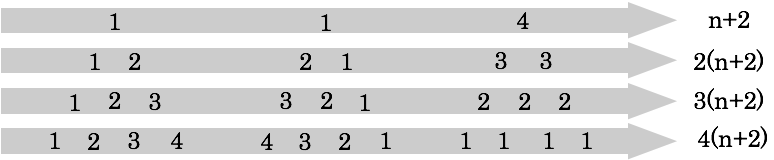
\includegraphics[scale=0.35]{FiguresArithmetic/appTetrahedral3}
        \caption{The basic pattern for computing $\widehat{\Theta}_n$ (for $n=4$).}
        \label{fig:Tetrahedral3}
\end{center}
\end{figure}
Because triangles have three sides, we have three ways to represent them---by rotating the sides in the manner of Fig.~\ref{fig:Tetrahedral1}.
\begin{figure}[h]
\begin{center}
        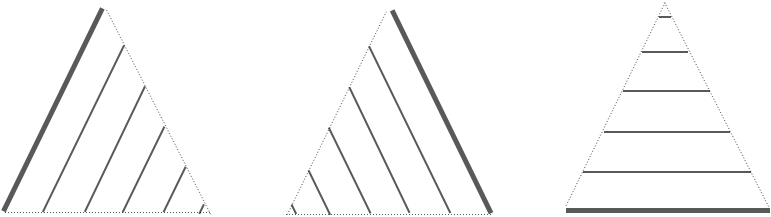
\includegraphics[scale=0.3]{FiguresArithmetic/appTetrahedral1}
        \caption{A schematic view of the three ways of organizing the triangles.
        The numbers are the same on each solid line: the bold one contains the $1$.}
        \label{fig:Tetrahedral1}
\end{center}
\end{figure}
Once we exploit these multiple views, we invoke Fubini's principle to sum up the successive rows of the figure.  Our strategy is guided by a search for an {\em invariant}.  In this case, we find that the sum of the elements along the rows of the three triangles is proportional to $n+2$.

Finally, we sum the numbers in each row in Fig.~\ref{fig:Tetrahedral4}.
\begin{figure}[h]
\begin{center}
        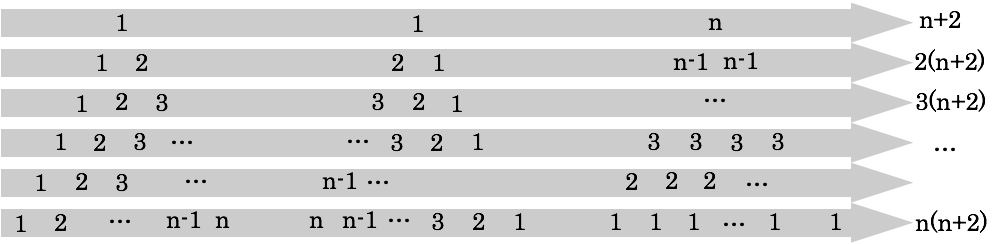
\includegraphics[scale=0.32]{FiguresArithmetic/appTetrahedral4}
        \caption{Detail of the computation of the invariant.}
        \label{fig:Tetrahedral4}
\end{center}
\end{figure}
\begin{itemize}
\item 
The sum along the first row is  $1+1+n \ = \ n+2$.
\item
The sum along the second row is $3 + 3 + 2 (n-1) \ = \ 2(n+2)$. 
\item
Let use sum up the elements in row $k$: 

$\Delta_k + \Delta_k + k(n-k+1) \ = \ k(k+1) \ + \ kn \ - \ k^2 \ + \ k \ = \  k(n+2)$.
\end{itemize}
Thus, the sum of all rows equals $\Delta_n \cdot (n+2)$.

\smallskip

But this summation has computed $\widehat{\Theta}_n$ three times!  We conclude that
%$= \frac{1}{4}.\widehat{\Theta}_n.(n+3)$
%The global sum is equal to $n+2$ times $(1+2+...+n)$.
\[ \widehat{\Theta}_n \ = \ {1 \over 3} \Delta_n \dot (n+2) \]
We thereby get a more intuitive path to the value of $\widehat{\Theta}_n$.

\medskip

\noindent \fbox{
\begin{minipage}{0.96\textwidth}
{\bf A summarizing note}.

\smallskip

It is important to recognize the natural progression in this section, because this will guide further extensions of these ideas.

We have thus far proved the following:
\[ \begin{array}{ccccccc}
Id_n & = & 1+1+ \cdots +1 & = & n \\
\Delta_n & = & 1+2+ \cdots +n & = & {1 \over 2} Id_n \cdot (n+1) & = & {1 \over 2} n (n+1) \\
\widehat{\Theta}_n & = & \Delta_1 + \Delta_2 + \cdots + \Delta_n & = & 
{1 \over 3} \Delta_n \cdot (n+2) & = & {1 \over 3!} n(n+1)(n+2)
\end{array} \]

With each increase in rank, we take one additional copy of the structure that characterizes the preceding rank:
\begin{itemize}
\item
With rank 1 ($Id_n$), we take {\em one} copy of $n$ tokens.

\medskip
\item
With rank 2 ($\Delta_n$), we take {\em two} copies of the $n$ tokens of rank 1, organized as triangles.

\medskip
\item
With rank 3 ($\widehat{\Theta}_n$), we take {\em three} copies of the triangles of rank 2, organized as tetrahedra.
\end{itemize} 
\end{minipage}
}
\medskip

We will end with a sketch of the next rank, the {\em Pentahedral numbers}.  You will be able to guess how to proceed at each step.


%%%%%%%%%%%%%%%%%%%%
\section{$\oplus$ Pentahedral Numbers}

\index{pentahedral number} \index{$\Pi_n$: the $n$th pentahedral number}

It is natural to ponder whether the regular patterns observed thus far will allow us to go to the next rank---to the {\em pentahedral numbers} 
\[ \Pi_n \ \eqdef \ \widehat{\Theta}_1 \ + \ \widehat{\Theta}_2 \ + \cdots + \ \widehat{\Theta}_n \]
Let's see \ldots

\medskip

Extrapolating from ranks $1$, $2$, and $3$, we would expect to encounter the following evaluation for the pentahedral number $\Pi_n$.
\[
\Pi_n \ = \ \widehat{\Theta}_1 + \widehat{\Theta}_2 + \cdots + \widehat{\Theta}_n \ = \
{1 \over 4} \widehat{\Theta}_n \cdot (n+3) \ = \ {1 \over 4!} n(n+1)(n+2)(n+3) 
\]
{\em In fact, this chain of equations is valid!}  The required direct algebraic manipulations---replacing the $\widehat{\Theta}_k$ by their expressions and simplifying---are a bit cumbersome but definitely doable.

\smallskip

It is not so easy to extend the pictorial construction.  However, we know that there should be four copies of $\widehat{\Theta}_n$ to consider.  So let us see where intuition leads us.

\smallskip

We organize three copies of $\widehat{\Theta}_n$ of them within the same triangular pattern in Fig.~\ref{fig:Tetrahedral6}.
\begin{figure}[h]
\begin{center}
        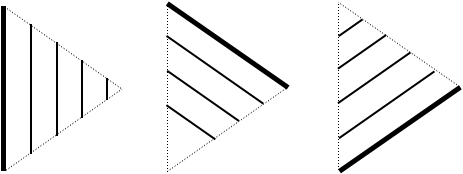
\includegraphics[scale=0.3]{FiguresArithmetic/appTetrahedral6}
        \caption{Computing $\Pi_n$: The three basic triangle patterns (solid lines represent integers with the same value).}
        \label{fig:Tetrahedral6}
\end{center}
\end{figure}

Because each element is a  copy of $\widehat{\Theta}_k$, let us decompose them again as we did in Fig.~\ref{fig:Tetrahedral7} (for $n=4$).  We arrive at Fig.~\ref{fig:Tetrahedral7}.
\begin{figure}[h]
\begin{center}
        \includegraphics[scale=0.35]{FiguresArithmetic/appTetrahedral7}
        \caption{Computing $\Pi_n$: Organizing the three basic triangle patterns (for $n=4$).}
        \label{fig:Tetrahedral7}
\end{center}
\end{figure}
Now, let us add the remaining copy of $\widehat{\Theta}_n$ in a manner that exposes an invariant.  As we found with lower ranks, we are able to find such an organization:
Summing within each row of the structure in Fig.~\ref{fig:Tetrahedral5} leads to an invariant: Each row sums to $n+3$
\begin{figure}[h]
\begin{center}
        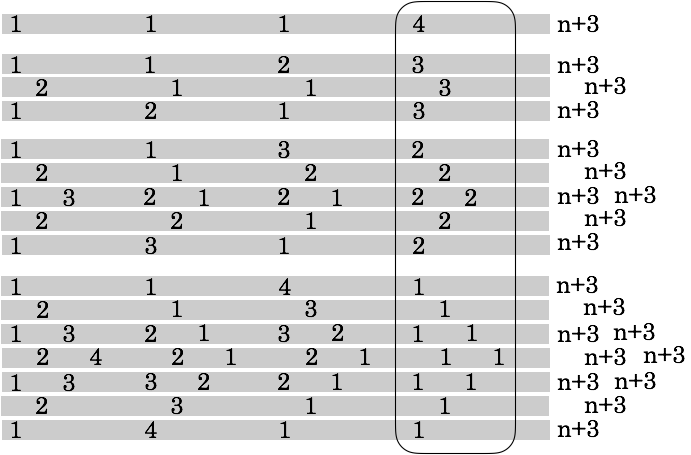
\includegraphics[scale=0.35]{FiguresArithmetic/appTetrahedral5}
        \caption{Add the last fourth copy of $\widehat{\Theta}_n$ and sum up the rows. The elements of the last column sum to $\widehat{\Theta}_n \cdot (n+3)$.}
        \label{fig:Tetrahedral5}
\end{center}
\end{figure}
The final result is now easy to obtain:
\begin{itemize}
\item 
The elements of the first row sum to $n+3$.
\item
The elements of the second series of rows sum to $3 (n+3)$. 
\item
The elements of the $k$th series of rows sum to $\Delta_k \cdot (n+3)$.
\end{itemize}
We thereby find that
\[
4 \Pi_n \ = \ (n+3) \cdot \sum_{k=1}^{n} \Delta_k \ = \ \widehat{\Theta}_n \cdot (n+3)
\]

\subsection{Can We Go Further?}

At this point, even the perspicuous pictorial summations become arduous.  We expect---but have not verified---that the hexahedral numbers, obtained by summing the first $n$ pentahedral numbers will sum to
\[ \sum_{k=1}^n \Pi_k \ = \ {1 \over 5} \Pi_n \cdot (n+4) \ = \ 
{1 \over 5!} n (n+1) (n+2) (n+3) (n+4)
\]

Are you up to the challenge?

